\documentclass[14pt, a4paper]{article}
\usepackage{minitoc}
\usepackage[left=3.00cm, right=2.5cm, top=2.00cm, bottom=2.00cm]{geometry}
\usepackage{amsmath}
\usepackage{amssymb}
\usepackage{amsthm}
\usepackage{thmtools}
\usepackage{mathtools}
\usepackage{graphicx}
%\usepackage{algpseudocode}
%\usepackage{algorithm}
\usepackage[ruled,vlined,linesnumbered,algosection]{algorithm2e}
\usepackage{blindtext}
\usepackage{setspace}
\usepackage[utf8]{inputenc}
\usepackage[utf8]{vietnam}
\usepackage[center]{caption}
\usepackage[shortlabels]{enumitem}
\usepackage{fancyhdr} % header, footer
\usepackage{hyperref} % loại bỏ border với mục lục và công thức
\usepackage[nonumberlist, nopostdot, nogroupskip]{glossaries}
\usepackage{glossary-superragged}
\usepackage{tikz,tkz-tab}
\setglossarystyle{superraggedheaderborder}
\pagestyle{fancy}
%\usepackage[style=numeric,sortcites]{biblatex}
%\addbibresource{ref.bib}
%\usepackage[numbers]{natbib}
\usepackage{indentfirst}
\usepackage{multirow}
\usepackage[natbib,backend=biber,style=ieee, sorting=ynt]{biblatex}
\bibliography{ref.bib}

\graphicspath{{./figures/}}


\makenoidxglossaries

% Danh mục thuật ngữ

\hypersetup{
    colorlinks=false,
    pdfborder={0 0 0},
}


\fancyhf{}
\rhead{\textbf{Môn học: Toán rời rạc và thuật toán}}
\lhead{\textbf{GVHD: PGS. TS. Nguyễn Thị Hồng Minh}}
\rfoot{\thepage}
\lfoot{\textbf{Nhóm học viên thực hiện: Nhóm 1}}
\renewcommand{\headrulewidth}{0.4pt}
\renewcommand{\footrulewidth}{0.4pt}


\numberwithin{equation}{section}
\numberwithin{figure}{section}

\setlength{\parindent}{0.5cm}

\setcounter{secnumdepth}{3} % Cho phép subsubsection trong report
\setcounter{tocdepth}{3} % Chèn subsubsection vào bảng mục lục

\newtheorem{dl}{Định lý}
\newtheorem{md}{Mệnh đề}
\newtheorem{bd}{Bổ đề}
\newtheorem{dn}{Định nghĩa}
\newtheorem{hq}{Hệ quả}

\numberwithin{dl}{section}
\numberwithin{md}{section}
\numberwithin{bd}{section}
\numberwithin{dn}{section}
\numberwithin{hq}{section}

\onehalfspacing
\AtBeginEnvironment{tabular}{\onehalfspacing}


\begin{document}
    \begin{titlepage}

        \newcommand{\HRule}{\rule{\linewidth}{0.5mm}} % Defines a new command for the horizontal lines, change thickness here

        \center % Center everything on the page

        %----------------------------------------------------------------------------------------
        %	HEADING SECTIONS
        %----------------------------------------------------------------------------------------
        \textsc{\LARGE Đại học Quốc Gia Hà Nội}\\[0.5cm]
        \textsc{\LARGE Trường đại học Khoa học tự nhiên}\\[0.5cm] % Name of your university/college
        \textsc{\LARGE Khoa Toán - Cơ - Tin học}\\[0.5cm]

        
\includegraphics[scale=0.2]{HUS-logo.jpg}\\[0.5cm]

        \textsc{\Large Chuyên ngành: Khoa học dữ liệu}\\[0.5cm] % Major heading such as course name


        %----------------------------------------------------------------------------------------
        %	TITLE SECTION
        %----------------------------------------------------------------------------------------

        \HRule \\[0.4cm]
        { \huge \bfseries BÁO CÁO CUỐI KỲ}\\[0.4cm] % Title of your document
        \HRule \\[1.5cm]

        \textsc{\Large Môn học: Toán rời rạc và thuật toán}\\[1cm] % Minor heading such as course title


        \textsc{\Large Đề tài: Lắp ghép các đoạn DNA \\ sử dụng tiếp cận của lý thuyết đồ thị}\\[1cm]


        %----------------------------------------------------------------------------------------
        %	AUTHOR SECTION
        %----------------------------------------------------------------------------------------
        \begin{minipage}{0.4\textwidth}
            \begin{flushleft} \large
            \emph{Giảng viên hướng dẫn:} \\
            PGS. TS. Nguyễn Thị Hồng Minh % Supervisor's Name
            \end{flushleft}
        \end{minipage}\\[0.5cm]

        \begin{minipage}{0.4\textwidth}
        \begin{flushleft} \large
        \emph{Nhóm học viên thực hiện:}\\
        Nguyễn Chí Thanh \\
        MSHV: 21007925 \\ % Your name
        Vũ Ngọc Đại \\
        MSHV: 21007977 \\
        Vũ Minh Hưng \\
        MSHV: 21007973 \\
        Lê Diệu Thúy \\
        MSHV: 21007922 \\
        Lớp: Khoa học dữ liệu - K4
        \end{flushleft}
        \end{minipage}


        % If you don't want a supervisor, uncomment the two lines below and remove the section above
        %\Large \emph{Author:}\\
        %John \textsc{Smith}\\[3cm] % Your name

        %----------------------------------------------------------------------------------------
        %	DATE SECTION
        %----------------------------------------------------------------------------------------

        % I don't want day because it is English
        % {\large \today}\\[2cm] % Date, change the \today to a set date if you want to be precise

        %----------------------------------------------------------------------------------------
        %	LOGO SECTION
        %----------------------------------------------------------------------------------------

        %\includegraphics{logo/rsz_3logo-khtn.png}\\[1cm] % Include a department/university logo - this will require the graphicx package

        %----------------------------------------------------------------------------------------

        \vfill % Fill the rest of the page with whitespace

    \end{titlepage}


    \cleardoublepage
    \pagenumbering{gobble}
    \tableofcontents
    \newpage
    \listoffigures
    \newpage
    \glsaddall 
    \renewcommand*{\glossaryname}{Danh mục các từ viết tắt}
    \renewcommand*{\acronymname}{Danh sách từ viết tắt}
    \renewcommand*{\entryname}{Viết tắt}
    \renewcommand*{\descriptionname}{Viết đầy đủ}
    \printnoidxglossary
    \cleardoublepage
    \pagenumbering{arabic}

    %\maketitle

    \newpage

    \nocite{*}

    \begin{center}
    \section*{LỜI MỞ ĐẦU}
    \end{center}
    \addcontentsline{toc}{section}{{\bf LỜI MỞ ĐẦU}\rm}

    Được xây dựng dựa trên các công trình trước đây về giải trình tự bằng lai ghép, lắp ráp các mảnh là một phương pháp mới được khám phá để xác định xem một chuỗi DNA được lắp ráp lại có khớp với chuỗi DNA ban đầu hay không.
    Một cách cụ thể để phân tích phương pháp này là sử dụng các khái niệm từ lý thuyết đồ thị.
    Bằng cách xây dựng các mô hình dữ liệu dựa trên những ý tưởng này, có thể đưa ra nhiều kết luận khác nhau về vấn đề ban đầu liên quan đến các chuỗi DNA được lắp ráp lại.
    Trong bài báo này ta sẽ trình bày chi tiết cách tiếp cận này để lắp ráp đoạn DNA và trình bày một số chứng minh lý thuyết trong quá trình lắp ráp bao gồm cả định lý BEST.
    Mặt khác, ta sẽ khám phá bài toán đường đi Euler và vai trò của nó trong việc hỗ trợ lắp ráp các đoạn DNA, và các ứng dụng khác gần đây của lý thuyết đồ thị trong lĩnh vực tin sinh học.

    \newpage
    \section{Mở đầu}
    
    Trong những năm gần đây, các nhà khoa học và các nhà nghiên cứu đã tập trung vào giải trình tự DNA và lắp ráp các đoạn với hy vọng nâng cao khả năng để tái tạo lại toàn bộ chuỗi DNA dựa trên các mảnh dữ liệu mà họ có thể thu được.
    Phức tạp nảy sinh khi lắp ráp các đoạn nhỏ do dữ liệu không hoàn hảo.
    Các sợi thường được lặp lại nhiều lần với nhiều độ dài khác nhau.
    Kết quả là, cấu hình của bộ gen ban đầu không hề dễ dàng như việc ghép mảnh này vào mảnh ghép tiếp theo.

    Ta sẽ thảo luận về các cách tiếp cận mới được khám phá gần đây để lắp ráp các đoạn DNA sử dụng các thành phần từ lý thuyết đồ thị,
    bao gồm đồ thị de Bruijin và chu trình Euler để khắc phục các sai lệch trong quá trình lắp ráp các đoạn DNA.
    Cụ thể, cách tiếp cận này bắt nguồn từ các công trình giải trình tự bằng lai ghép, bao gồm xây dựng các đồ thị có hướng dựa trên dữ liệu DNA được cung cấp và đếm số chu trình Euler trong các đồ thị này.

    Bài báo này sẽ cung cấp một số thông tin cơ bản sơ bộ từ lý thuyết đồ thị.
    Ngoài một số định nghĩa, ta sẽ chứng minh hai định lý, định lý BEST và định lý cây ma trận, cả hai đều được sử dụng trong việc đếm số chu trình Euler trong đồ thị có hướng.

    Hơn nữa, bài báo sẽ khảo sát ngắn gọn tình hình nghiên cứu của bài toán giải trình tự DNA và lắp ráp các đoạn DNA,
    chẳng hạn các vấn đề phát sinh và cách chúng được giải quyết bằng lý thuyết đồ thị.
    Ta sẽ xem cách các đồ thị được xây dựng sử dụng dữ liệu DNA và cách mà các đồ thị này biểu diễn bài toán.
    Vấn đề chính mà ta quan tâm là bài toán đường đi Euler trong \cite{pevzner2001eulerian}, \cite{pevzner2001new}, đây là một nỗ lực gần đây để đơn giản hóa đồ thị DNA thông qua một chuỗi các phép biến đổi trên đồ thị.
    Các phép biến đổi như vậy bao gồm các phép tách cạnh khác nhau cho các trường hợp có một và nhiều cạnh trong đồ thị Euler có hướng.

    Phần kết luận thảo luận sự phân tích của trình tự DNA với nanopores, như được trình bày chi tiết trong \cite{bokhari2005parallel} và vai trò của lý thuyết độ thị trong việc giải quyết các vấn đề nảy sinh.
    Đây là một ứng dụng gần đây hơn của lý thuyết đồ thị được đưa vào sử dụng trong lĩnh vực tinh sinh học.
    
    \section{Các định nghĩa trong lý thuyết đồ thị}

    Lý thuyết đồ thị là một lĩnh vực của toán học có nhiều ứng dụng trong thế giới khoa học.
    Ta giả định người đọc đã quen thuộc với những nền tảng cơ bản của lý thuyết đồ thị, chẳng hạn như được đề cập trong \cite{tucker2006applied} và \cite{west2001introduction}.
    Các thuật ngữ cơ bản trong bài báo theo các thuật ngữ của \cite{west2001introduction}.

    Ta có thẻ di chuyển qua các phần tử của đồ thị theo nhiều cách khác nhau.
    Một đường đi là một hành trình bất kỳ qua một đồ thị tạo ra một danh sách các đỉnh và các cạnh sao cho một cạnh kết nối các đỉnh ở hai bên của cạnh này.
    Một vết là một đường đi mà không có bất kỳ cạnh nào được lặp lại.
    Một vết khép kín là một chu trình và danh sách các đỉnh được biểu diễn theo thứ tự tuần hoàn.
    Hơn nữa, một đường dẫn là một vết mà trong đó không có đỉnh nào được lặp lại sao cho các đỉnh có thể được liệt kê theo thứ tự liên tiếp từ đỉnh này liền kề với đỉnh tiếp theo.
    Trong trường hợp đồ thị có hướng, các cạnh của một vết hoặc một chu trình phải nhất quán về hướng.

    Một vết hoặc một chu trình đi qua các cạnh trong đồ thị một lần và chính xác một lần được gọi là Euler.
    Các vết hoặc các chu trình Euler được cho phép đi qua các đỉnh trong đồ thị nhiều hơn một lần.
    Số chu trình Euler trong đồ thị có thể được tính toán với công thức từ định lý BEST, định lý này sẽ được chứng minh ở phần sau trong bài báo.

    Một định nghĩa cuối cùng từ lĩnh vực lý thuyết đồ thị mà ta sử dụng trong bài báo là đồ thị de Bruijin.
    Đồ thị de Bruijin là một đồ thị có hướng với các đỉnh biểu diễn các chuỗi ký tự từ bảng chữ cái và các cạnh cho biết vị trí mà chuỗi có thể chồng lên nhau như được định nghĩa trong \cite{de1946combinatorial}.

    Việc xây dựng đồ thị này phụ thuộc vào một tập các mảnh hoặc các đoạn có độ dài $l$ từ dãy cụ thể hiện có.
    Mỗi đỉnh được gán nhãn bởi một đoạn có chiều dài $l-1$ và cạnh có hướng tồn tại giữa hai đỉnh đại diện cho một trong đoạn có chiều dài $l$.
    Cụ thể, ký hiệu đầu tiên trong đoạn xuất phát từ đỉnh gửi cạnh và tương tự, ký tự cuối cùng biểu diễn đỉnh nhận.
    Vì vậy, các ký tự còn lại trong cả hai đỉnh bao gồm sẽ đánh dấu các cạnh.

    \begin{figure}[h!]
        \centering
        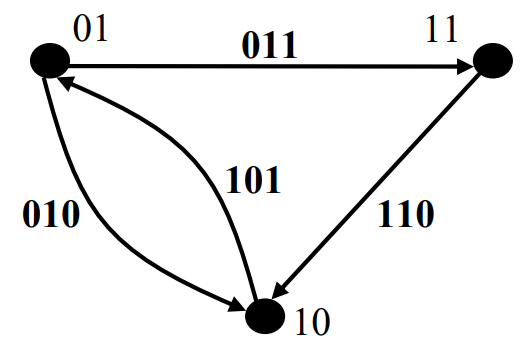
\includegraphics[width=0.4\textwidth]{1.png}
        \caption{Một đồ thị de Bruijin cho chuỗi "0110101" với các đoạn chiều dài là 3.}
        \label{fig:1}
    \end{figure}


    \newpage
    \printbibliography[title={TÀI LIỆU THAM KHẢO}]

\end{document}